% Chapter Template

\chapter{Mathematical Modelling} % Main chapter title

\label{Chapter2} % Change X to a consecutive number; for referencing this chapter elsewhere, use \ref{ChapterX}

\lhead{Chapter 2. \emph{Mathematical Modelling}} % Change X to a consecutive number; this is for the header on each page - perhaps a shortened title

%----------------------------------------------------------------------------------------
%	SECTION 1
%----------------------------------------------------------------------------------------
introduction to the problem... discussing a trivial problem    
\section{Mathematical Preliminaries}

%-----------------------------------
%	SUBSECTION 1
%-----------------------------------
The modelling of a system requires understanding the ... \citep{craig2009introduction}.  

content here ...
\newpage % avoid it in between chapters 

\subsection{Rotation Matrices}
The configuration of a point is completely described by its position vector in $\mathbb{R}^3$, whereas for a rigid body, the orientation of the body in space also needs to be defined.
The orientation of a body-fixed frame $B$ with respect to a reference frame $A$ as shown in Fig. \ref{fig:trans} is given by $R_{AB}$. The rotation matrix that transforms the coordinate frame \textit{A} to coordinate frame \textit{B} has the property:

\begin{equation}\label{eq:ortho}
R_{AB}^{\intercal}\cdot R_{AB} = \mathbb{I}_{3\times 3}.
\end{equation}

\begin{figure}[!htb]
    \centering
    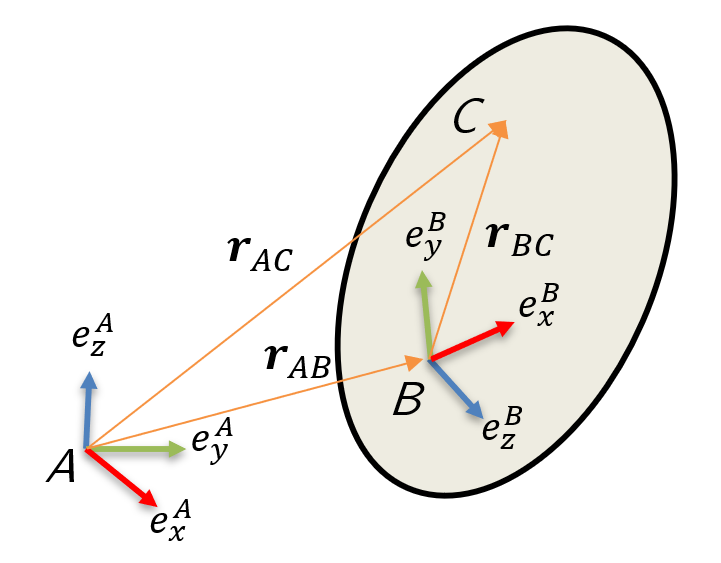
\includegraphics[scale=0.45]{trans_T.PNG}
    \caption{ Coordinate transformations for a single rigid body}
    \label{fig:trans}
\end{figure}

Further, the rotation matrix belongs to a special orthonormal group $SO(3)$, and has properties $R_{AB}^{-1} = R_{BA} = R_{AB}^{\intercal}$.

The orientation of a body could be parametrized in many ways. There are a total of nine parameters in a $3 \times 3$ rotation matrix, but they are constrained by the orthogonality condition of Eq. \ref{eq:ortho}. There are only three independent parameters, and Euler angles are used for a minimal representation of rotations in space.

%----------------------------------------------------------------------------------------
%	SECTION 2
%----------------------------------------------------------------------------------------
